\documentclass[a4paper]{article}
\usepackage[T1]{fontenc}
\usepackage[utf8]{inputenc}
\usepackage[italian]{babel}
\usepackage{amsmath}
\usepackage{amsfonts}
\usepackage{amssymb}
\usepackage{resizegather} \addtolength{\jot}{4pt}
\usepackage{graphicx}
\usepackage{booktabs}
\usepackage{caption}
	\captionsetup{tableposition=top,figureposition=bottom,font=small}
	\captionsetup{format=hang,labelfont={sf,bf}}
\usepackage{subfig}
\usepackage{siunitx}
	\sisetup{output-exponent-marker=\ensuremath{\mathrm{e}}}
\usepackage{quoting}
	\quotingsetup{font=small}
\usepackage{hyperref}
	\hypersetup{hidelinks}
\usepackage{url}
\usepackage{pgfplots}
	\pgfplotsset{compat=newest}
\usepackage{microtype}

\renewcommand{\vec}[1]{\mathbf{#1}}
\DeclareMathOperator{\diver}{div}
\newcommand{\bhat}{\hat{\vec{b}}}
\newcommand{\bigO}[1]{\mathcal{O}\!\left(#1\right)}
\newcommand{\dx}{\, dx}
\newcommand{\dgamma}{\, d\gamma}
\newcommand{\pluseq}{\mathrel{+}=}
\newcommand{\norm}[1]{\left\lVert#1\right\rVert}
\newcommand{\norminf}[1]{\left\lVert#1\right\rVert_\infty}
\newcommand{\normtwo}[1]{\left\lVert#1\right\rVert_2}
\newcommand{\normltwo}[1]{\left\lVert#1\right\rVert_{L^2}}
\newcommand{\normhone}[1]{\left\lVert#1\right\rVert_{H^1}}
\newcommand{\R}{\mathbb{R}}
\newcommand{\seminorm}[1]{\left\lvert#1\right\rvert}

\title{\huge{Elaborato per l'esame di \\
Complementi di Analisi Numerica}}
\author{\Large{Bruno Degli Esposti}}
\date{Luglio 2019}

\begin{document}

\maketitle

\begin{abstract}
In questo elaborato ho cercato sia di approfondire alcuni argomenti
visti a lezione, sia di esporre le conoscenze di FreeFEM che ho acquisito
con il seminario della professoressa Falini,
la Modelling Week di Madrid e qualche giorno di studio individuale.
L'elaborato è diviso in tre parti.
La prima parte consiste in un confronto tra il metodo delle differenze finite
e il metodo degli elementi finiti per la soluzione dell'equazione di
Laplace su una corona circolare con condizioni al bordo di Dirichlet.
La seconda parte consiste nella soluzione di un problema ADR con condizioni
al bordo miste in cui il termine convettivo domina su quello diffusivo.
Ho confrontato l'efficacia di varie tecniche di stabilizzazione,
come il metodo upwind e streamline-diffusion.
La terza parte consiste nell'applicazione del $\theta$-metodo per la soluzione
dell'equazione del calore con condizioni al bordo di Robin.
Il codice relativo al metodo delle differenze finite (FDM) è stato sviluppato
con MATLAB, mentre quello relativo al metodo degli elementi finiti (FEM)
è stato sviluppato con FreeFEM.
\end{abstract}

\tableofcontents

\section{Equazione di Laplace}
Ho scelto il seguente problema per confrontare i due metodi:
\begin{equation} \label{eqn:laplace-cartesiano}
\begin{cases}
\Delta u(x,y) = 0 \quad & \text{in $\Omega \subseteq \mathbb{R}^2$} \\
u(x,y) = f(x,y)   \quad & \text{su $\partial \Omega$ regolare}
\end{cases}
\end{equation}
Il dominio $\Omega$ è una corona circolare centrata
nell'origine, con raggio interno $1$ e raggio esterno $2$.
La funzione $f$ è armonica, così da risultare essa stessa soluzione del problema.
Questo permetterà in seguito di calcolare con precisione l'errore
commesso dai due metodi. Ho scelto
\[
f = \operatorname{Re}\left(\frac{1}{z}\right) = \frac{x}{x^2+y^2}
\]
È immediato verificare che $f$ sia armonica, in quanto parte reale di
una funzione olomorfa su $\Omega$.

\subsection{Metodo delle differenze finite}
Per poter applicare il metodo delle differenze finite,
è necessario innanzitutto trovare un mapping da un rettangolo
di $\R^2$ a $\Omega$.
Questo problema è in generale difficile da risolvere,
ma in questo caso basta passare alle coordinate polari $\rho$ e $\theta$.
Sia $g$ l'espressione di $f$ in queste coordinate, ovvero
$g \colon (\rho, \theta) \mapsto f(\rho\cos(\theta), \rho\sin(\theta))$.
L'analogo del problema~\eqref{eqn:laplace-cartesiano} in
coordinate polari è il seguente:
\begin{equation} \label{eqn:laplace-polare}
\begin{cases}
\frac{\partial^2 v}{\partial\rho^2}
	+ \frac{1}{\rho} \frac{\partial v}{\partial\rho}
	+ \frac{1}{\rho^2} \frac{\partial^2 v}{\partial\theta^2} = 0
	\qquad & \text{in $\Psi = (1,2)\times(0,2\pi) \subseteq \mathbb{R}^2$} \\
v(1,\theta) = g(1,\theta)
	\qquad & \text{per ogni $\theta \in [0,2\pi]$} \\
v(2,\theta) = g(2,\theta)
	\qquad & \text{per ogni $\theta \in [0,2\pi]$} \\
v(\rho,0) = g(\rho,2\pi)
	\qquad & \text{per ogni $\rho \in [1,2]$} \\
\end{cases}
\end{equation}
Dopo aver cambiato dominio, è comparso nell'equazione differenziale
un termine di trasporto orizzontale in $\Psi$, radiale in $\Omega$.
Il rapporto tra il coefficiente di trasporto e quello di diffusione
non supera $1$ su tutto $\Psi$, pertanto non si rende
necessaria l'applicazione di uno schema upwind.
Sono cambiate anche le condizioni al bordo,
adesso miste tra Dirichlet e periodiche.

Ora che il problema~\eqref{eqn:laplace-cartesiano} è stato riformulato
in modo da avere come dominio un rettangolo, si può procedere
con la definizione di una griglia $G$ su $\Psi$.
Siano $N_\rho$ e $N_\theta$ il numero di suddivisioni uniformi
rispettivamente lungo $\rho$ e lungo $\theta$. Allora
\[
G = \{ (1+(i-1)/N_\rho, \; 2\pi (j-1)/N_\theta)
\mid i = 1,\dots,N_\rho+1 \quad j = 1,\dots,N_\theta \}.
\]
Gli indici partono da $1$ e non da $0$ per rispettare la convenzione di MATLAB.
Siano $h_\rho$ e $h_\theta$ i passi di discretizzazione orizzontali
e verticali della griglia, cioé $1/N_\rho$ e $2\pi/N_\theta$.
Dalla griglia sono stati esclusi i punti con $\theta = 2\pi$, perché la
condizione al bordo periodica li rende superflui (basta usare al loro posto
i punti con $\theta = 0$).
In seguito sarà utile pensare a $G$ anche come vettore di~$\R^N$,
dove $N = |G| = (N_\rho+1)N_\theta$. In tal caso verrà utilizzato $k$
come indice monodimensionale, al posto di $i$ e $j$.
La funzione contenuta nel file \texttt{get\_k.m} permette di calcolare $k$ a partire
da $i$, $j$ e $N_\theta$.

A questo punto si può applicare il metodo delle differenze finite
per trasformare il problema continuo~\eqref{eqn:laplace-polare}
in un problema discreto della forma $A_h v_h = b_h$, ovvero
un sistema lineare $N$-dimensionale.
Una volta risolto tale sistema, l'elemento $k$-esimo di $v_h$
è l'approssimazione di $v(G_k)$ fornita dal metodo.
C'è da dire che in questo caso non si può applicare
nessuno dei teoremi visti a lezione circa
%l'esistenza e unicità della soluzione del problema \eqref{eqn:laplace-polare},
l'esistenza dell'inversa di $A_h$
o l'uniforme limitatezza della norma di $A_h^{-1}$.
Per fortuna, entrambe le proprietà continuano a valere,
come ho potuto verificare numericamente.
In particolare, per quanto riguarda la stabilità del metodo, ho ottenuto
la seguente stima empirica:
\[
\norminf{A_h^{-1}} \leq M, \quad \text{con $M \approx 1.13$ per ogni $h > 0$.}
\]
Per quanto riguarda invece la consistenza del metodo, l'errore di
troncamento locale $\tau_h$ è sicuramente in $\bigO{h_\rho^2 + h_\theta^2}$,
perché ho scelto di usare il metodo delle differenze finite centrate
del secondo ordine e la soluzione $f$ ha la regolarità
richiesta (è addirittura analitica). Dunque mi aspetto che
\[
\norminf{e_h} = \norminf{v_h-v} \in \bigO{h^2},
\quad \text{con $h = \sqrt{h_\rho^2 + h_\theta^2}$.}
\]
Fissato un punto $(\rho_i, \theta_j)$ interno a $G$, diciamo $G_k$,
la $k$-esima equazione lineare del sistema $A_h v_h = b_h$ è
\begin{equation} \label{eqn:fdm}
\begin{gathered}
\frac{v_h(\rho_{i+1},\theta_j)
    -2v_h(\rho_{i},  \theta_j)
     +v_h(\rho_{i-1},\theta_j)}{h_\rho^2}
+\frac{1}{\rho_i}
 \frac{v_h(\rho_{i+1},\theta_j)-v_h(\rho_{i-1},\theta_j)}{2h_\rho} \\[6pt]
+\frac{1}{\rho_i^2}
 \frac{v_h(\rho_i,\theta_{j+1})
     -2v_h(\rho_i,\theta_j)
      +v_h(\rho_i,\theta_{j-1})}{h_\theta^2} = 0
\end{gathered}
\end{equation}
Se invece $(\rho_i, \theta_j)$ appartiene al bordo di $G$,
l'equazione precedente va modificata in modo opportuno;
i dettagli sono presenti all'interno del codice.
Ho trovato utile scrivere l'equazione \eqref{eqn:fdm} anche sotto forma di tabella:
\begin{equation*}
\resizebox{\linewidth}{!}
{$
\displaystyle \sum
\begin{bmatrix}
&
\left(\frac{1}{\rho_i^2} \frac{1}{h_\theta^2}\right)
	v_h(\rho_i,\theta_{j+1})
& \\[8pt]
\left( \frac{1}{h_\rho^2} - \frac{1}{\rho_i} \frac{1}{2h_\rho} \right)
	v_h(\rho_{i-1},\theta_j) &
\left( -\frac{2}{h_\rho^2} - \frac{1}{\rho_i^2} \frac{2}{h_\theta^2} \right)
	v_h(\rho_i,\theta_j)     &
\left( \frac{1}{h_\rho^2} + \frac{1}{\rho_i} \frac{1}{2h_\rho} \right)
	v_h(\rho_{i+1},\theta_j) \\[8pt]
&
\left( \frac{1}{\rho_i^2} \frac{1}{h_\theta^2} \right) v_h(\rho_i,\theta_{j-1})
& \end{bmatrix} = 0
$}
\end{equation*}
Il codice MATLAB per la soluzione del problema~\eqref{eqn:laplace-polare}
%mediante il metodo delle differenze finite centrate del secondo ordine
è contenuto nel file \texttt{differenze\_finite.m}.
Ho preferito imporre la condizione al bordo di Dirichlet tramite diagonalizzazione,
senza eliminare gradi di libertà. Mi pare che il codice risulti così più chiaro.

\subsection{Metodo degli elementi finiti}
Anche per il metodo degli elementi finiti è necessario riformulare
il problema~\eqref{eqn:laplace-cartesiano}. Occorre infatti
costruire una triangolazione regolare $\mathcal{T}_h$ di~$\Omega$ e trasformare
l'equazione di Laplace dalla forma forte alla forma debole.
Per quanto riguarda la generazione della mesh regolare, questa viene effettuata in
automatico da FreeFEM a partire da una parametrizzazione di~$\partial\Omega$,
in questo caso due circonferenze.
Per avere un confronto significativo con il metodo delle differenze finite,
il numero di suddivisioni delle circonferenze in segmenti verrà nuovamente
indicato con~$N_\theta$.
A partire da queste suddivisioni e dai vertici così fissati,
viene generata una triangolazione di Delaunay all'interno,
con una densità di vertici proporzionale a quella sul bordo.
La documentazione di FreeFEM descrive così il procedimento:
\begin{quoting}
A triangulation is built by the keyword \texttt{buildmesh}.
This keyword calls a triangulation subroutine based on the Delaunay test,
which first triangulates with only the boundary points,
then adds internal points by subdividing the edges.
How fine the triangulation becomes is controlled by the size
of the closest boundary edges.
\end{quoting}
Una volta generata la triangolazione $\mathcal{T}_h$,
si può passare alla definizione di $V_h$.
FreeFEM non usa la tecnica di rilevamento del dato sul bordo:
il vincolo costituito dalle condizioni di Dirichlet viene imposto tramite
penalizzazione durante la fase di algebra lineare.
Pertanto all'interno del codice l'insieme $V_h$ coincide con tutto $X_h^r$.
Questo aspetto è messo in luce in modo inequivocabile dal fatto che,
nel caso di elementi lineari, la dimensione di $V_h$ è uguale al
numero di vertici della mesh, compresi quelli sul bordo.
Un'altra peculiarità di FreeFEM è che $V_h$, una volta definito
con il comando \texttt{fespace}, diventa un nuovo tipo di dato.
Così, almeno da un punto di vista sintattico, basta assegnare $f$ a
una variabile di tipo $V_h$ per trovare la proiezione di $f$ su $V_h$. Molto comodo!

Per quanto riguarda la formulazione variazionale, basta moltiplicare
l'equazione di Laplace per una funzione test $v \in V = H_0^1(\Omega)$,
integrare su $\Omega$ e applicare il teorema della divergenza:
\[
0
= - \int_\Omega{\Delta u v \dx}
= - \int_{\partial\Omega}{\frac{\partial u}{\partial \mathbf{n}} v \dgamma}
  + \int_\Omega{\nabla u \cdot \nabla v \dx}
=   \int_\Omega{\nabla u \cdot \nabla v \dx}
= a(u,v)
\]
In questo caso il funzionale lineare $F(v)$ è nullo.
Indichiamo con $\{\varphi_i\}$ gli elementi della base lagrangiana di $V_h$.
Seguendo il metodo di Galerkin, FreeFEM può ora assemblare la matrice
di stiffness $A_h$ e il vettore di carico $f_h$:
\[
(A_h)_{ij} = a(\varphi_i,\varphi_j) \qquad (f_h)_i = F(\varphi_i) = 0
\]
Una volta calcolati $A_h$ e $f_h$, FreeFEM apporta loro delle modifiche
tramite il comando \texttt{on}, che serve a imporre le condizioni al bordo
di Dirichlet tramite penalizzazione.
Per ogni elemento $\varphi_i$ che vale 1 su un punto base $P_i$ appartenente
al bordo della mesh, si pone
\[
(A_h)_{ii} \pluseq \texttt{tgv}, \qquad
(f_h)_i \pluseq f(P_i) \cdot \texttt{tgv}, \qquad
\text{con $\texttt{tgv} = 10^{30}$ di default.}
\]
In questo modo la soluzione $u_h$ del sistema lineare $A_h u_h = f_h$ soddisfa
a precisione di macchina la condizione $(u_h)_i = f(P_i)$.
Ho trovato utile a riguardo la lettura del paragrafo \textit{A.2 Imposing essential boundary conditions},
in appendice al testo di Formaggia, Saleri, Veneziani.

La soluzione $u$ del problema \eqref{eqn:laplace-cartesiano} è analitica,
quindi $u \in H^{r+1}(\Omega)$ e vale la seguente stima dell'errore
per il metodo degli elementi finiti:
\[
\normhone{u-u_h} \leq \frac{M}{\alpha} C h^r \seminorm{u}_{r+1}
\]

Di default, FreeFEM usa il metodo iterativo GMRES per risolvere il sistema lineare.
Visto che in questo caso la matrice $A_h$ è simmetrica definita positiva,
ho provato anche a usare il metodo dei gradienti coniugati.
Non ho però ottenuto alcun beneficio, pur scegliendo adeguatamente le tolleranze.
In ogni caso, il metodo iterativo scelto non usa precondizionamento.

\subsection{Confronto tra FDM e FEM}
Le figure \ref{fig:pb1-solution-FD-20} e \ref{fig:pb1-solution-FE-20} mostrano
l'aspetto delle soluzioni numeriche ottenute con i due metodi per $N_\theta = 126$.
Purtroppo il software di visualizzazione incluso in FreeFEM ha delle serie limitazioni,
ovvero non permette l'output in formato vettoriale
o l'ingrandimento della legenda che riporta i valori delle curve di livello.
%Per confrontare ... ho scelto elementi finiti lagrangiani di ordine $r = 1$ o $r = 2$.
Le tabelle \ref{tab:Pb1 FD results}, \ref{tab:Pb1 FE P1 results}
e \ref{tab:Pb1 FE P2 results} indicano in dettaglio i risultati ottenuti con i
vari metodi, rispettivamente differenze finite del second'ordine,
elementi finiti lineari ed elementi finiti quadratici.
La colonna $t_a$ riporta il numero di secondi richiesto per l'assemblaggio
del sistema lineare, includendo nel caso degli elementi finiti il costo
di generazione della mesh. La colonna $t_s$ riporta invece il tempo
richiesto dalla fase di algebra lineare.
Nelle tabelle \ref{tab:Pb1 FD results} e \ref{tab:Pb1 FE P1 results}, il numero di
vertici della mesh e la dimensione del sistema lineare coincidono.
Ho riportato pertanto solo quest'ultimo valore.
Nella tabella \ref{tab:Pb1 FE P2 results} non ho riportato le informazioni
su $h$, perché coincidono con quelle della tabella \ref{tab:Pb1 FE P1 results}.
Infatti i due metodi FE, anche se di ordine diverso, usano la stessa mesh
a parità di $N_\theta$. Un esempio di tale mesh per $N_\theta = 63$
è riportato in figura \ref{fig:Pb1 Mesh FE 10}.
Per quanto riguarda il metodo delle differenze finite,
la figura \ref{fig:Pb1 Mesh FD 10} mostra la griglia $G$ a cui
è stato applicato il mapping delle coordinate polari.

Ottenere anche solo una cifra significativa corretta nelle stime numeriche
degli errori per il metodo degli elementi finiti si è rivelato veramente difficile.
Alla fine, ho ottenuto risultati soddisfacenti solo nel seguente modo:
\begin{itemize}
\item Ho generato una triangolazione di riferimento $\mathcal{T}_{ref}$ molto fitta.
\item Ho proiettato $u$ su $V_{ref}$, spazio degli elementi P4 su $\mathcal{T}_{ref}$.
\item Ho elevato $u_h$ da $V_h$ a $V_{ref}$.
\item Ho calcolato $\norm{u_h - u}$ usando formule di quadratura di ordine 10.
\end{itemize}
I dettagli sono presenti all'interno del codice. Senza questi accorgimenti,
cioé lavorando direttamente in $V_h$, ho ottenuto stime fino a due ordini
di grandezza più piccole. Talvolta gli errori non avevano nemmeno
un andamento monotono rispetto a $h$.
Dall'analisi dei dati riportati, emergono le seguenti considerazioni:
\begin{itemize}
\item Nel codice MATLAB, il tempo $t_a$ richiesto per l'assemblaggio aumenta
	con il quadrato del numero di vertici della mesh, il che significa che ho scritto
	un programma poco efficiente. La colpa va attribuita senz'altro al modo in cui viene
	costruita $A_h$. Ho preallocato in memoria una matrice sparsa CSC con \texttt{spalloc()}
	e poi ho assegnato tutti i valori \texttt{v} alle entrate non nulle con
	la sintassi \texttt{Ah(k,l) = v}.
	La documentazione di MATLAB suggerisce invece di costruire prima i tre vettori
	della rappresentazione COO di $A_h$, poi di chiamare la funzione \texttt{sparse()},
	con cui si ottiene la forma CSC.
\item Nel codice FreeFEM, il tempo $t_a$ richiesto per l'assemblaggio aumenta
	linearmente con il numero di vertici della mesh, il che è ottimale.
	Nel caso di elementi lineari, la fase di assemblaggio costa
	più della soluzione del sistema lineare (di un 25\% circa).
	Nel caso di elementi quadratici,
	è la fase di algebra lineare a costare di più (oltre il doppio).
\item Per il metodo delle differenze finite, l'andamento asintotico
	della norma infinito dell'errore è effettivamente $\bigO{h^2}$,
	in accordo con la teoria.
	Si osservi a riguardo la figura \ref{fig:Pb1 Comparison Inf}.
	Nella stessa figura si può vedere come anche il metodo degli elementi finiti
	presenti il medesimo andamento asintotico dell'errore, sia per $r = 1$ che per $r = 2$.
	In questo caso non conosco risultati teorici di riferimento.
	
	Per il metodo delle differenze finite, l'errore è calcolato in modo puntuale
	sui vertici della griglia $G$.
	Per il metodo FEM, invece, ho cercato di dare una stima su tutto $\mathcal{T}_h$.
	Tale stima è circa 10 volte più grande di quella che avrei potuto ottenere
	confrontando i valori solo sui punti base della triangolazione.
	A bilanciare questa scelta, riducendo le stime, c'è il fatto che nel
	grafico~\ref{fig:Pb1 Comparison Inf} ho riportato i valori $h_{max}$ delle mesh,
	e non delle ipotetiche medie~$h_{avg}$.
	
	In conclusione, direi che i metodi FD e FEM con elementi quadratici
	forniscono soluzioni della stessa qualità,
	per quel che riguarda l'errore in norma infinito.
	Il metodo FD richiede però la soluzione di un sistema lineare più piccolo,
	quindi in questo caso mi sembra preferibile (si confrontino le colonne $t_s$).
\item Per il metodo degli elementi finiti, l'andamento asintotico
	della norma $H^1$ dell'errore è effettivamente $\bigO{h^r}$,
	in accordo con la teoria.
	Si osservi a riguardo la figura \ref{fig:Pb1 Comparison L2 and H1}.
	Nella stessa figura si può vedere anche l'andamento della norma $L^2$
	dell'errore. Trovo interessante il fatto che nel caso di elementi finiti quadratici,
	$\normltwo{e}$ vada a zero come $h^{2.5}$, anziché $h^{3}$.
\item La famiglia $\mathcal{F}$ di triangolazioni generata da FreeFEM è quasi-uniforme,
	perché il rapporto tra $h_{min}$ e $h_{max}$ è limitato inferiormente da $0.26$ circa.
\end{itemize}

\begin{table}[p]
\caption{Metodo delle differenze finite}
\label{tab:Pb1 FD results}
\centering
\resizebox{\linewidth}{!}{
\begin{tabular}{cccccccc}
\toprule
$N_\theta$ & $h$ & $\norminf{e}$ & $\normltwo{e}$ & $\normhone{e}$ &
$\dim(A_h)$ & $t_a$ & $t_s$ \\
\midrule
63  & \num{1.41e-1} & \num{2.57e-4} & - & - & 693   & \num{2.5e-3} & \num{1.6e-3} \\ %10
88  & \num{1.01e-1} & \num{1.32e-4} & - & - & 1320  & \num{5.3e-3} & \num{3.0e-3} \\ %14
126 & \num{7.06e-2} & \num{6.52e-5} & - & - & 2646  & \num{1.4e-2} & \num{7.9e-3} \\ %20
176 & \num{5.05e-2} & \num{3.33e-5} & - & - & 5104  & \num{3.8e-2} & \num{1.7e-2} \\ %28
251 & \num{3.53e-2} & \num{1.63e-5} & - & - & 10291 & \num{1.2e-1} & \num{3.8e-2} \\ %40
358 & \num{2.48e-2} & \num{8.05e-6} & - & - & 20764 & \num{4.1e-1} & \num{7.3e-2} \\ %57
503 & \num{1.77e-2} & \num{4.09e-6} & - & - & 40743 & \num{1.5e+0} & \num{1.6e-1} \\ %80
710 & \num{1.25e-2} & \num{2.05e-6} & - & - & 80940 & \num{7.1e+0} & \num{3.6e-1} \\ %113
\bottomrule
\end{tabular}
}
\end{table}

\begin{table}[p]
\caption{Metodo degli elementi finiti P1}
\label{tab:Pb1 FE P1 results}
\centering
\resizebox{\linewidth}{!}{
\begin{tabular}{ccccccccc}
\toprule
$N_\theta$ & $h_{max}$ & $\frac{h_{min}}{h_{max}}$ & $\norminf{e}$ & $\normltwo{e}$ &
$\normhone{e}$ & $\dim(A_h)$ & $t_a$ & $t_s$ \\
\midrule
63  & \num{2.82e-1} & 0.30 & \num{5.30e-3} & \num{3.16e-3} & \num{1.48e-1} & 510   & \num{7.0e-3} & \num{7.0e-3} \\ %10
88  & \num{2.00e-1} & 0.30 & \num{2.56e-3} & \num{1.57e-3} & \num{1.04e-1} & 983   & \num{1.3e-2} & \num{9.0e-3} \\ %14
126 & \num{1.41e-1} & 0.27 & \num{1.24e-3} & \num{7.75e-4} & \num{7.25e-2} & 1986  & \num{2.7e-2} & \num{1.7e-2} \\ %20
176 & \num{1.02e-1} & 0.26 & \num{6.72e-4} & \num{4.05e-4} & \num{5.22e-2} & 3705  & \num{4.9e-2} & \num{3.3e-2} \\ %28
251 & \num{7.04e-2} & 0.26 & \num{3.25e-4} & \num{1.96e-4} & \num{3.60e-2} & 7695  & \num{1.0e-1} & \num{7.8e-2} \\ %40
358 & \num{4.95e-2} & 0.27 & \num{1.52e-4} & \num{9.63e-5} & \num{2.52e-2} & 15138 & \num{2.1e-1} & \num{1.6e-1} \\ %57
503 & \num{3.54e-2} & 0.27 & \num{8.57e-5} & \num{4.68e-5} & \num{1.73e-2} & 32517 & \num{4.7e-1} & \num{3.8e-1} \\ %80
710 & \num{2.52e-2} & 0.27 & \num{3.91e-5} & \num{2.52e-5} & \num{1.27e-2} & 57982 & \num{9.7e-1} & \num{7.0e-1} \\ %113
\bottomrule
\end{tabular}
}
\end{table}

\begin{table}[p]
\caption{Metodo degli elementi finiti P2}
\label{tab:Pb1 FE P2 results}
\centering
\resizebox{\linewidth}{!}{
\begin{tabular}{cccccccc}
\toprule
$N_\theta$ & $\norminf{e}$ & $\normltwo{e}$ &
$\normhone{e}$ & vertici & $\dim(A_h)$ & $t_a$ & $t_s$ \\
\midrule
63  & \num{6.22e-4} & \num{1.27e-4} & \num{2.71e-2} & 505   & 1894   & \num{9.0e-3} & \num{1.7e-2} \\ %10
88  & \num{3.19e-4} & \num{4.54e-5} & \num{1.39e-2} & 983   & 3756   & \num{1.7e-2} & \num{3.4e-2} \\ %14
126 & \num{1.55e-4} & \num{1.60e-5} & \num{6.73e-3} & 1986  & 7692   & \num{3.5e-2} & \num{7.4e-2} \\ %20
176 & \num{7.90e-5} & \num{6.41e-6} & \num{3.43e-3} & 3705  & 14468  & \num{6.1e-2} & \num{1.5e-1} \\ %28
251 & \num{3.92e-5} & \num{2.41e-6} & \num{1.66e-3} & 7695  & 30278  & \num{1.3e-1} & \num{3.5e-1} \\ %40
358 & \num{1.89e-5} & \num{9.83e-7} & \num{7.92e-4} & 15138 & 59836  & \num{2.7e-1} & \num{7.8e-1} \\ %57
503 & \num{9.75e-6} & \num{4.12e-7} & \num{3.78e-4} & 32517 & 129062 & \num{6.9e-1} & \num{1.8e+0} \\ %80
710 & \num{4.87e-6} & \num{1.77e-7} & \num{1.77e-4} & 57982 & 230508 & \num{1.3e+0} & \num{3.5e+0} \\ %113
\bottomrule
\end{tabular}
}
\end{table}

\begin{figure}
\centering
\begin{tikzpicture}
\begin{loglogaxis}[xlabel={Passo di discretizzazione $h$}, ylabel=Errore $\norminf{e}$,
                   width=\textwidth, height=0.8\textheight,
                   legend style={anchor=north west,at={(0.04,0.97)}}]
\addplot[green!60!black,mark=*] coordinates
{(0.141, 2.57e-4) (0.101, 1.32e-4) (0.070, 6.52e-5) (0.051, 3.33e-5)
(3.53e-2, 1.63e-5) (2.48e-2, 8.05e-6) (1.77e-2, 4.09e-6) (1.25e-2, 2.05e-6)}; % FD einf
\addplot[blue,mark=*] coordinates
{(2.82e-1, 5.30e-3) (2.00e-1, 2.56e-3) (1.41e-1, 1.24e-3) (1.02e-1, 6.72e-4)
(7.04e-2, 3.25e-4) (4.95e-2, 1.52e-4) (3.54e-2, 8.57e-5) (2.52e-2, 3.91e-5)}; % FE P1 einf
\addplot[red,mark=*] coordinates
{(2.82e-1, 6.22e-4) (2.00e-1, 3.19e-4) (1.41e-1, 1.55e-4) (1.02e-1, 7.90e-5)
(7.04e-2, 3.92e-5) (4.95e-2, 1.89e-5) (3.54e-2, 9.75e-6) (2.52e-2, 4.87e-6)}; % FE P2 einf
\addplot[loosely dashed, domain=1e-2:0.2] {1e-1*x^2};
\addplot[dashed,         domain=1e-2:0.2] {1e-2*x^2};
\legend{Differenze finite, Elementi finiti P1, Elementi finiti P2,
        $0.1 \cdot h^2$, $0.01 \cdot h^2$}
\end{loglogaxis}
\end{tikzpicture}
\caption{Confronto degli errori in norma infinito.}
\label{fig:Pb1 Comparison Inf}
\end{figure}

\begin{figure}
\centering
\begin{tikzpicture}
\begin{loglogaxis}[xlabel={Passo di discretizzazione $h$}, ylabel=Errore $\normltwo{e}$ e $\normhone{e}$,
                   ymin = 2e-9, ymax = 5e-1,
                   width=\textwidth, height=0.9\textheight,
                   legend style={anchor=south east,at={(0.96,0.03)}}]
\addplot[blue,mark=*] coordinates
{(2.82e-1, 3.16e-3) (2.00e-1, 1.57e-3) (1.41e-1, 7.75e-4) (1.02e-1, 4.05e-4)
(7.04e-2, 1.96e-4) (4.95e-2, 9.63e-5) (3.54e-2, 4.68e-5) (2.52e-2, 2.52e-5)}; % P1 L2
\addplot[cyan,mark=*] coordinates
{(2.82e-1, 1.48e-1) (2.00e-1, 1.04e-1) (1.41e-1, 7.25e-2) (1.02e-1, 5.22e-2)
(7.04e-2, 3.60e-2) (4.95e-2, 2.52e-2) (3.54e-2, 1.73e-2) (2.52e-2, 1.27e-2)}; % P1 H1
\addplot[red,mark=*] coordinates
{(2.82e-1, 1.27e-4) (2.00e-1, 4.54e-5) (1.41e-1, 1.60e-5) (1.02e-1, 6.41e-6)
(7.04e-2, 2.41e-6) (4.95e-2, 9.83e-7) (3.54e-2, 4.12e-7) (2.52e-2, 1.77e-7)}; % P2 L2
\addplot[orange,mark=*] coordinates
{(2.82e-1, 2.71e-2) (2.00e-1, 1.39e-2) (1.41e-1, 6.73e-3) (1.02e-1, 3.43e-3)
(7.04e-2, 1.66e-3) (4.95e-2, 7.92e-4) (3.54e-2, 3.78e-4) (2.52e-2, 1.77e-4)}; % P2 H1
\addplot[loosely dashed, domain=1e-2:0.2] {3e-1*x^1};
\addplot[dashed,         domain=1e-2:0.2] {1e-1*x^2};
\addplot[densely dashed, domain=1e-2:0.2] {1e-2*x^2.5};
\legend{$\normltwo{e}$ per elementi P1, $\normhone{e}$ per elementi P1,
        $\normltwo{e}$ per elementi P2, $\normhone{e}$ per elementi P2,
        $0.3 \cdot h^1$, $0.1 \cdot h^2$, $0.01 \cdot h^{2.5}$}
\end{loglogaxis}
\end{tikzpicture}
\caption{Confronto degli errori in norma $L^2$ e $H^1$.}
\label{fig:Pb1 Comparison L2 and H1}
\end{figure}

\begin{figure}
\centering
\subfloat[][Differenze finite \label{fig:Pb1 Mesh FD 10}]
	{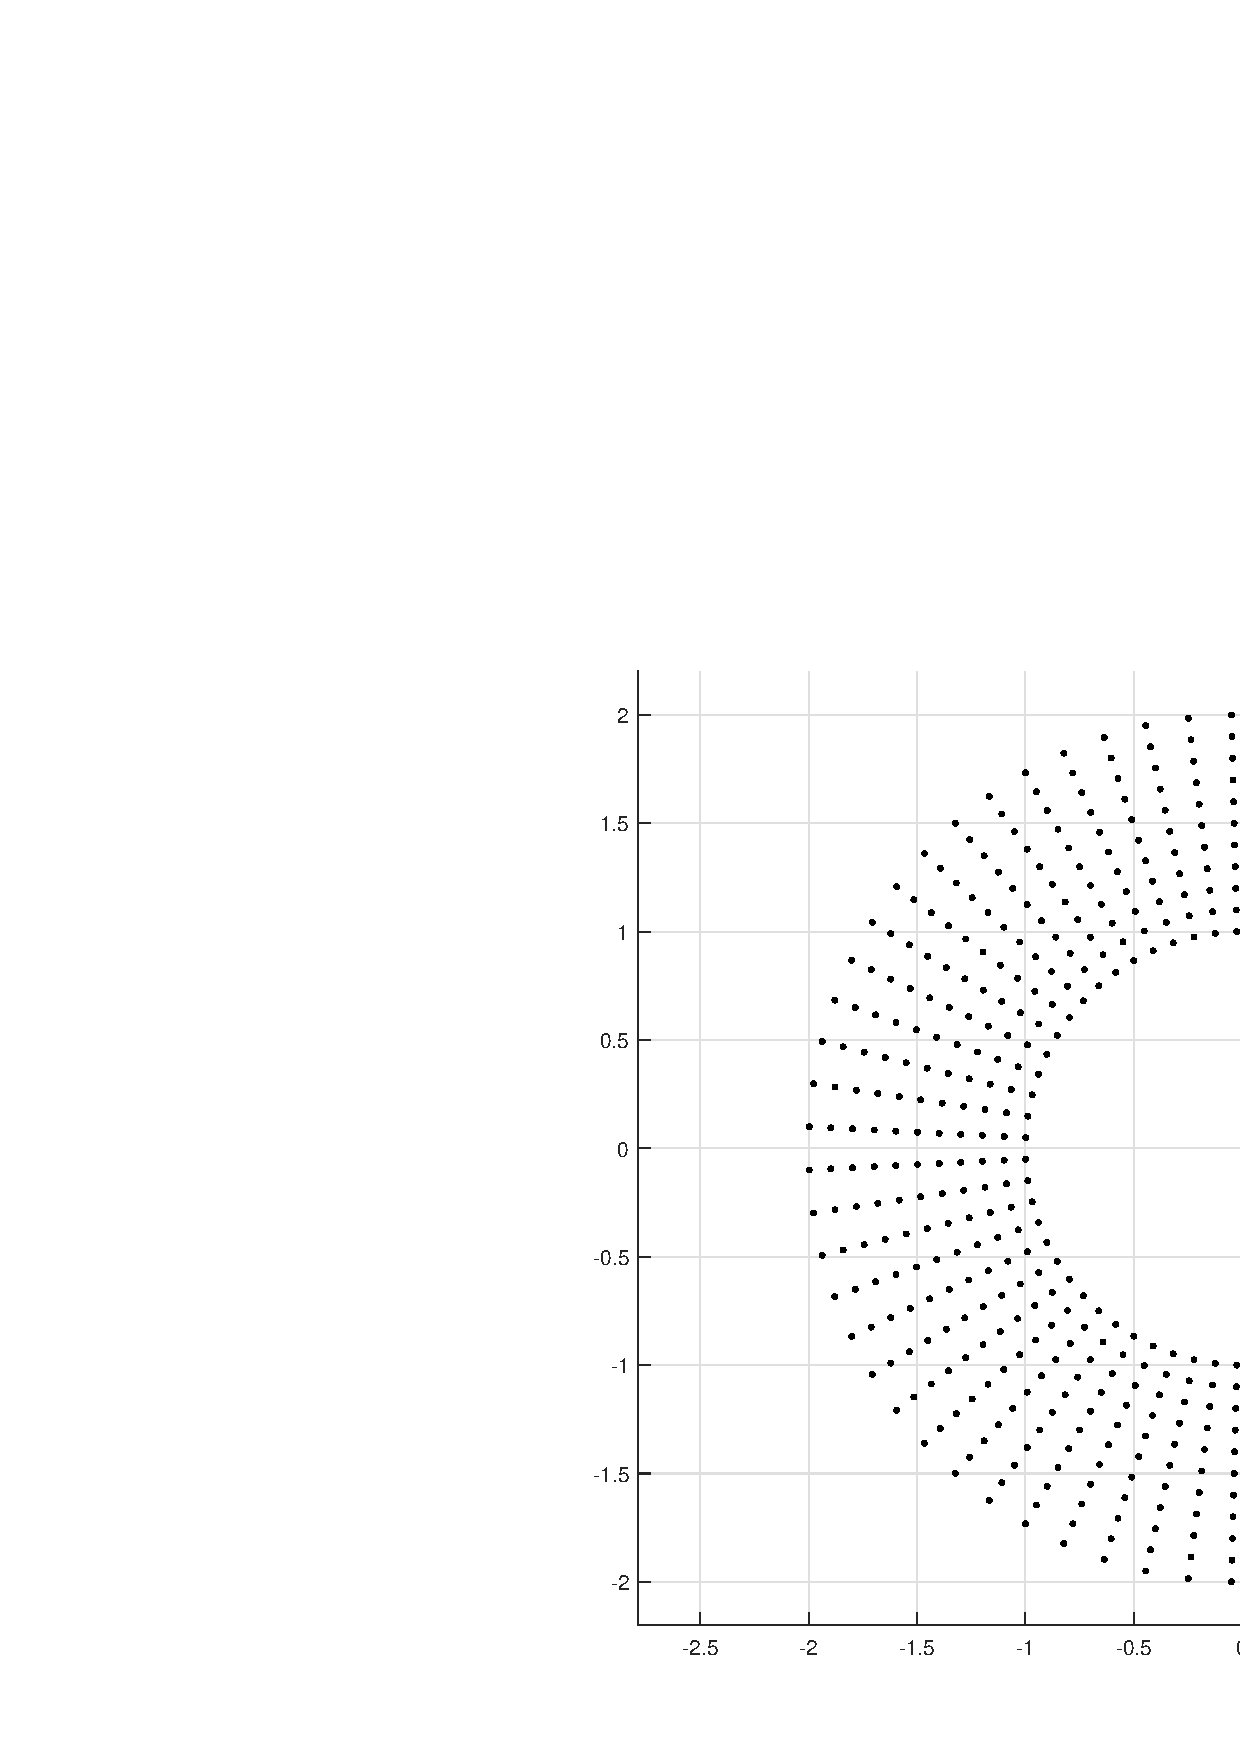
\includegraphics[height=0.23\textheight]{figures/mesh_FD_10.png}} \quad
\subfloat[][Elementi finiti \label{fig:Pb1 Mesh FE 10}]
	{\includegraphics[height=0.22\textheight]{figures/mesh_FE_10.png}}
\caption{Mesh a confronto con $N_\theta = 10$.}
\label{fig:subfig}
\end{figure}

\begin{figure}
\centering
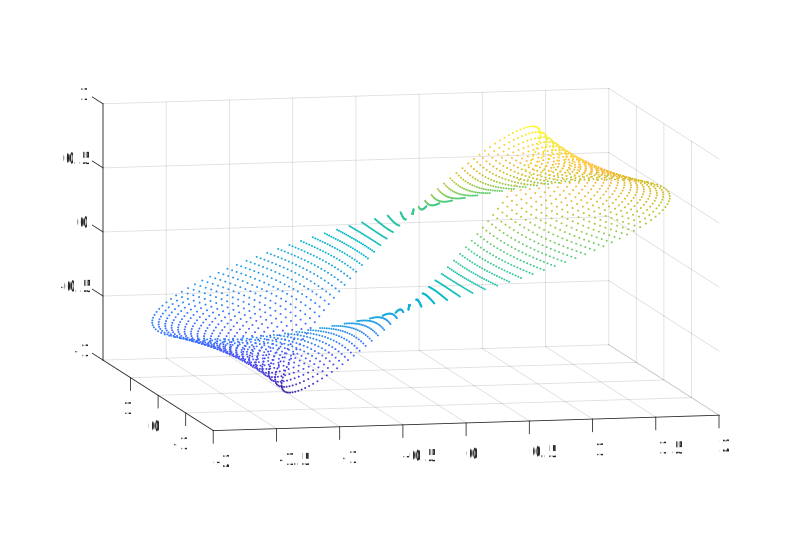
\includegraphics[width=0.9\textwidth]{figures/solution_FD_20.png}
\caption{Soluzione FDM, con $N_\theta = 20$.}
\label{fig:pb1-solution-FD-20}
\end{figure}

\begin{figure}
\centering
\includegraphics[width=0.8\textwidth]{figures/solution_FE_20.png}
\caption{Soluzione FEM P2, con $N_\theta = 20$.}
\label{fig:pb1-solution-FE-20}
\end{figure}

\clearpage

\section{Problema ADR}
Si consideri il seguente problema di diffusione-trasporto-reazione:
\begin{equation} \label{eqn:ADR-strong}
\begin{cases}
- \mu \Delta u + \vec{b} \cdot \nabla u + \sigma u = 0
\quad & \text{in $\Omega \subseteq \mathbb{R}^2$} \\
u = 1 \quad & \text{su $\Gamma_1 \subseteq \partial \Omega$} \\
\frac{\partial u}{\partial \vec{n}} = 0 \quad & \text{su $\Gamma_2 \subseteq \partial \Omega$} \\
u = -1 \quad & \text{su $\Gamma_3 \subseteq \partial \Omega$} \\
\frac{\partial u}{\partial \vec{n}} = 0 \quad & \text{su $\Gamma_4 \subseteq \partial \Omega$}
\end{cases}
\end{equation}
Il dominio $\Omega$ è un trapezio con vertici $\{(-1,3),(-1,-3),(1,-1),(1,1)\}$.
Le porzioni di bordo $\Gamma_1,\dots,\Gamma_4$ corrispondono a lati del trapezio
come in figura. \vspace{6pt}

\begin{figure}[h]
\centering
\begin{tikzpicture}
\begin{axis}[xlabel={$x$}, ylabel={$y$}, xmin = -5, xmax = 5, ymin = -5, ymax = 5,
	         grid=major, height=0.25\textheight, ylabel style={rotate=-90}]
                   %legend style={anchor=south east,at={(0.96,0.03)}}]
\addplot[black,mark=*] coordinates
{(-1,3) (-1,-3) (1,-1) (1,1) (-1,3)};
\node[left,black] at (-1.5,0) {$\Gamma_1$};
\node[below,black] at (0.5,-2.5) {$\Gamma_2$};
\node[right,black] at (1.5,0) {$\Gamma_3$};
\node[above,black] at (0.5,2.5) {$\Gamma_4$};

\end{axis}
\end{tikzpicture}
\caption{Il dominio $\Omega$ e il suo bordo.}
\label{fig:pb2-omega}
\end{figure}

I coefficienti $\mu$, $\vec{b}$ e $\sigma$ sono costanti, per semplicità.
All'interno del codice, queste costanti sono state scelte in modo da garantire
esistenza e unicità della soluzione.
Sono anche state scelte affinché si formi uno strato limite nei pressi di~$\Gamma_3$,
a causa del termine di trasporto $\vec{b}$ che domina su quello di diffusione~$\mu$.
Per il problema \eqref{eqn:ADR-strong} non ho previsto nessuna soluzione
in forma chiusa con cui confrontare i risultati numerici ottenuti.
Ho cercato pertanto di calcolare con FreeFEM una soluzione numerica
di riferimento con la più alta accuratezza possibile.
A tal fine, ho trovato utile la funzione \texttt{adaptmesh()}, che permette di
rendere la mesh più fitta in corrispondenza dello strato limite.

\subsection{Formulazione variazionale}
Siano $\Gamma_D = \Gamma_1 \cup \Gamma_3$, $\Gamma_N = \Gamma_2 \cup \Gamma_4$
e $v \in H_D^1(\Omega)$. Allora si ha che
\begin{gather*}
- \int_\Omega{\mu \Delta u v \dx}
+ \int_\Omega{(\vec{b} \cdot \nabla u) v \dx}
+ \int_\Omega{\sigma u v \dx} = 0 \\
%%%
- \int_{\partial\Omega}{\mu \frac{\partial u}{\partial \mathbf{n}} v \dgamma}
+ \int_\Omega{\mu \nabla u \cdot \nabla v \dx}
+ \int_\Omega{(\vec{b} \cdot \nabla u) v \dx}
+ \int_\Omega{\sigma u v \dx} = 0 \\
%%%
- \int_{\Gamma_D}{\mu \frac{\partial u}{\partial \mathbf{n}} v \dgamma}
- \int_{\Gamma_N}{\mu \frac{\partial u}{\partial \mathbf{n}} v \dgamma}
+ \int_\Omega{\mu \nabla u \cdot \nabla v \dx}
+ \int_\Omega{(\vec{b} \cdot \nabla u) v \dx}
+ \int_\Omega{\sigma u v \dx} = 0 \\
%%%
- \int_{\Gamma_D}{\mu \frac{\partial u}{\partial \mathbf{n}} 0 \dgamma}
- \int_{\Gamma_N}{\mu \, 0 \, v \dgamma}
+ \int_\Omega{\mu \nabla u \cdot \nabla v \dx}
+ \int_\Omega{(\vec{b} \cdot \nabla u) v \dx}
+ \int_\Omega{\sigma u v \dx} = 0 \\
%%%
a(u,v) - F(v)
= \int_\Omega{\mu \nabla u \cdot \nabla v \dx}
+ \int_\Omega{(\vec{b} \cdot \nabla u) v \dx}
+ \int_\Omega{\sigma u v \dx}
= 0
\end{gather*}

\subsection{Tecniche di stabilizzazione}
La soluzione ottenuta con il metodo di Galerkin standard
\[
\textit{Calcolare $u_h$ tale che $a(u_h,v_h) = F(v_h)$ per ogni $v_h \in V_h$}
\]
può presentare oscillazioni spurie, se il numero di Peclet locale
\[
Pe = \frac{\normtwo{\vec{b}}h}{2\mu}
\]
è maggiore di 1. Una rimedio consiste nello scegliere
$h < 2\mu/\normtwo{\vec{b}}$, ma se $\normtwo{\vec{b}} \gg \mu$
il costo associato al calcolo della soluzione può essere proibitivo.
A lezione sono state presentate due tecniche che permettono di recuperare
il corretto andamento qualitativo della soluzione senza dover ridurre $h$:
la \emph{diffusione artificiale} e la \emph{streamline-diffusion}.
Il fondamento teorico di entrambe le tecniche consiste nel
metodo di Galerkin generalizzato
\begin{gather*}
\textit{Calcolare $u_h$ tale che $a(u_h,v_h) + b_h(u_h,v_h)$} \\
\textit{$= F(v_h) + G_h(v_h)$ per ogni $v_h \in V_h$}
\end{gather*}
in cui $b_h(u_h,v_h)$ e $G_h(v_h)$ sono detti
\emph{termini di stabilizzazione}.
Nel caso della diffusione artificiale upwind, si ha
\[
b_h(u_h,v_h) = \mu Pe \int_\Omega{\nabla u_h \cdot \nabla v_h \dx} \qquad G_h(v_h) = 0
\]
Questa scelta risulta equivalente all'aggiunta di $-\mu Pe \Delta u$ nell'equazione
differenziale associata al probema \eqref{eqn:ADR-strong}.
L'ordine di convergenza che si ottiene è~$\bigO{h}$ indipendentemente da $r$.
La diffusione artificiale di tipo Scharfetter-Gummel è analoga alla precedente,
con la differenza che al numero di Peclet locale viene applicata la funzione
\[
\varphi(t) = t - 1 + B(2t), \qquad \text{con $B(t) =$}
\begin{cases}
\frac{t}{e^t - 1} & \text{se $t > 0$} \\
1                 & \text{se $t = 0$}
\end{cases}
\]
L'ordine di convergenza migliora e diventa $\min\{r,2\}$.
Sia $\bhat$ il vettore $\vec{b}$ normalizzato.
Nel caso della streamline-diffusion, si pone
\[
b_h(u_h,v_h) =
- \mu Pe \int_{\Gamma_N}{(\nabla u_h \cdot \bhat) (\vec{n} \cdot \bhat) v_h \dgamma}
+ \mu Pe \int_\Omega{(\nabla u_h \cdot \bhat) (\nabla v_h \cdot \bhat) \dx}
\]
Questa scelta corrisponde all'aggiunta di
$-\mu Pe \, \diver((\nabla u \cdot \bhat) \, \bhat)$
nell'equazione differenziale associata al probema \eqref{eqn:ADR-strong}.
Per dimostrarlo, basta ripetere il procedimento utilizzato per passare alla
formulazione variazionale:
\begin{gather*}
- \int_\Omega{\mu \Delta u v \dx}
- \int_\Omega{\mu Pe \, \diver((\nabla u \cdot \bhat) \, \bhat) v \dx}
+ \int_\Omega{(\vec{b} \cdot \nabla u) v \dx}
+ \int_\Omega{\sigma u v \dx} = 0 \\
%%%
\dots
- \mu Pe \int_{\partial \Omega}{(\nabla u \cdot \bhat) (\vec{n} \cdot \bhat) v \dgamma}
+ \mu Pe \int_\Omega{(\nabla u \cdot \bhat) (\nabla v \cdot \bhat) \dx}
+ \dots = 0 \\
%%%
\dots
- \mu Pe \int_{\Gamma_N}{(\nabla u \cdot \bhat) (\vec{n} \cdot \bhat) v \dgamma}
+ \mu Pe \int_\Omega{(\nabla u \cdot \bhat) (\nabla v \cdot \bhat) \dx}
+ \dots = 0
\end{gather*}
L'ordine di convergenza che si ottiene è~$\bigO{h}$ indipendentemente da $r$,
ma in linea di principio aver aggiunto viscosità solamente nella direzione di $\vec{b}$
dovrebbe portare a soluzioni più accurate rispetto alla tecnica upwind.
Anche per la streamline-diffusion si può scegliere di applicare $\varphi$ a $Pe$,
portando così l'ordine di convergenza a $\min\{r,2\}$.

\subsection{Confronto dei risultati}
La figura \ref{fig:pb2-results} permette di confrontare l'aspetto qualitativo
di alcune soluzioni numeriche che ho ottenuto con i programmi
\texttt{adr\_galerkin\_standard.edp}, \texttt{adr\_upwind.edp}
e \texttt{adr\_streamline\_diffusion.edp}.
Ho scelto i seguenti parametri per il problema:
\[
\mu = 1 \qquad \vec{b} = (30,0) \qquad \sigma = 1
\]
Si noti come il metodo di Galerkin standard presenti
forti oscillazioni nei pressi dello strato limite.
%per i valori di $h$ indicati in didascalia.
La soluzione ottenuta con il metodo della viscosità artificiale upwind
presenta invece un andamento monotòno, sicuramente più vicino a quello della
soluzione numerica di riferimento (che ai fini della stima dell'errore
viene considerata come se fosse esatta).

Purtroppo, non sono riuscito a replicare i risultati di
convergenza teorici che ho riassunto nella sottosezione precedente.
In particolare, ho notato che la qualità della soluzione migliora in modo
marginale nel passaggio da elementi finiti lineari a elementi finiti quadratici.
Sospetto quindi che la soluzione debole $u$ di questo problema ADR
non abbia la regolarità $H^2(\Omega)$ richiesta dalle stime di interpolazione
alla base dei risultati teorici.
La mancanza di regolarità potrebbe essere dovuta alle condizioni al bordo miste,
o alla geometria particolare di $\Omega$ con due angoli interni di $\ang{135}$.

Le tabelle \ref{tab:pb2-galerkin-standard}, \ref{tab:pb2-upwind}
e \ref{tab:pb2-streamline-diffusion} indicano in dettaglio i risultati ottenuti con il
metodo degli elementi finiti P1 al variare delle tecniche di stabilizzazione.
La colonna $\sup e$ riporta il valore massimo assunto dalla funzione $u_h - u$.
Delle tante quantità possibili per rilevare la presenza di oscillazioni nella
soluzione, questa è risultata la più affidabile tra quelle che ho provato.
% no phi(pe)
Dall'analisi dei dati riportati, emergono le seguenti considerazioni:
\begin{itemize}
\item Quando il numero di Peclet locale è grande,
	sono i metodi stabilizzati a presentare l'errore più piccolo.
	Quando invece $Pe$ scende sotto una certa soglia (intorno a 3),
	il metodo di Galerkin standard torna a essere più accurato.
	Le oscillazioni non scompaiono del tutto (si osservi la colonna $\sup e$),
	ma si smorzano abbastanza da confondersi con il restante profilo dell'errore.
\item L'ordine di convergenza del metodo risulta inferiore a 1,
	ammesso che la soluzione di riferimento sia attendibile.
	Si vede bene nella figura \ref{fig:pb2-confronto} come le curve
	degli errori tendano ad allontanarsi dalla retta di riferimento tratteggiata,
	invece che proseguire in parallelo.
\item Per questo problema (in particolare direi per questo dominio $\Omega$)
	la tecnica di streamline-diffusion sembra non apportare alcun tipo
	di beneficio rispetto alla diffusione artificiale upwind.
	Anzi, il sistema lineare associato risulta leggermente più costoso da risolvere.
\end{itemize}

\begin{table}[p]
\caption{Metodo degli elementi finiti P1 standard}
\label{tab:pb2-galerkin-standard}
\centering
\begin{tabular}{ccccccc}
\toprule
$h$ & $Pe$ & $\normhone{e}$ & $\sup{e}$ & $\dim(A_h)$ & $t_a$ & $t_s$ \\
\midrule
\num{5.00e-1} & \num{7.50e+0} & \num{1.22e+1} & \num{1.97e+0} & 67     & \num{1.0e-3} & \num{2.0e-3} \\
\num{3.54e-1} & \num{5.30e+0} & \num{1.05e+1} & \num{1.38e+0} & 137    & \num{2.0e-3} & \num{1.0e-3} \\
\num{2.50e-1} & \num{3.75e+0} & \num{9.12e+0} & \num{1.07e+0} & 230    & \num{3.0e-3} & \num{2.0e-3} \\
\num{1.77e-1} & \num{2.65e+0} & \num{6.92e+0} & \num{5.92e-1} & 511    & \num{5.0e-3} & \num{7.0e-3} \\
\num{1.25e-1} & \num{1.87e+0} & \num{5.48e+0} & \num{4.10e-1} & 892    & \num{9.0e-3} & \num{1.1e-2} \\
\num{8.84e-2} & \num{1.33e+0} & \num{4.19e+0} & \num{2.24e-1} & 1599   & \num{1.6e-2} & \num{2.1e-2} \\
\num{6.25e-2} & \num{9.37e-1} & \num{3.08e+0} & \num{1.28e-1} & 3305   & \num{3.3e-2} & \num{4.5e-2} \\
\num{4.42e-2} & \num{6.63e-1} & \num{2.29e+0} & \num{6.14e-2} & 6856   & \num{7.3e-2} & \num{1.0e-1} \\
\num{3.12e-2} & \num{4.69e-1} & \num{1.69e+0} & \num{3.97e-2} & 13167  & \num{1.6e-1} & \num{2.2e-1} \\
\num{2.21e-2} & \num{3.31e-1} & \num{1.28e+0} & \num{1.84e-2} & 25765  & \num{3.1e-1} & \num{4.2e-1} \\
\num{1.56e-2} & \num{2.34e-1} & \num{9.30e-1} & \num{8.52e-3} & 52104  & \num{6.8e-1} & \num{9.2e-1} \\
\num{1.10e-2} & \num{1.66e-1} & \num{7.04e-1} & \num{4.33e-3} & 104038 & \num{1.5e+0} & \num{2.0e+0} \\
\bottomrule
\end{tabular}
\end{table}

\begin{table}[p]
\caption{Metodo degli elementi finiti P1 con viscosità artificiale upwind}
\label{tab:pb2-upwind}
\centering
\begin{tabular}{cccccc}
\toprule
$h$ & $\normhone{e}$ & $\sup{e}$ & $\dim(A_h)$ & $t_a$ & $t_s$ \\
\midrule
\num{5.00e-1} & \num{9.77e+0} & \num{6.13e-3} & 67     & \num{1.0e-3} & \num{2.0e-3} \\
\num{3.54e-1} & \num{9.19e+0} & \num{4.97e-3} & 137    & \num{2.0e-3} & \num{1.0e-3} \\
\num{2.50e-1} & \num{8.58e+0} & \num{3.92e-3} & 230    & \num{3.0e-3} & \num{2.0e-3} \\
\num{1.77e-1} & \num{7.64e+0} & \num{2.88e-3} & 511    & \num{6.0e-3} & \num{6.0e-3} \\
\num{1.25e-1} & \num{6.73e+0} & \num{2.09e-3} & 892    & \num{9.0e-3} & \num{1.1e-2} \\
\num{8.84e-2} & \num{5.73e+0} & \num{1.50e-3} & 1599   & \num{1.7e-2} & \num{2.2e-2} \\
\num{6.25e-2} & \num{4.71e+0} & \num{1.06e-3} & 3305   & \num{3.5e-2} & \num{4.8e-2} \\
\num{4.42e-2} & \num{3.78e+0} & \num{7.54e-4} & 6856   & \num{7.2e-2} & \num{1.0e-1} \\
\num{3.12e-2} & \num{2.96e+0} & \num{5.33e-4} & 13167  & \num{1.4e-1} & \num{2.0e-1} \\
\num{2.21e-2} & \num{2.28e+0} & \num{3.76e-4} & 25765  & \num{2.9e-1} & \num{4.2e-1} \\
\num{1.56e-2} & \num{1.71e+0} & \num{2.65e-4} & 52104  & \num{6.5e-1} & \num{9.0e-1} \\
\num{1.10e-2} & \num{1.28e+0} & \num{1.87e-4} & 104038 & \num{1.5e+0} & \num{2.0e+0} \\
\bottomrule
\end{tabular}
\end{table}

\begin{table}[p]
\caption{Metodo degli elementi finiti P1 con streamline-diffusion}
\label{tab:pb2-streamline-diffusion}
\centering
\begin{tabular}{cccccc}
\toprule
$h$ & $\normhone{e}$ & $\sup{e}$ & $\dim(A_h)$ & $t_a$ & $t_s$ \\
\midrule
\num{5.00e-1} & \num{9.77e+0} & \num{3.60e-4} & 67     & \num{1.0e-3} & \num{2.0e-3} \\
\num{3.54e-1} & \num{9.21e+0} & \num{1.12e-3} & 137    & \num{1.0e-3} & \num{2.0e-3} \\
\num{2.50e-1} & \num{8.60e+0} & \num{1.11e-3} & 230    & \num{2.0e-3} & \num{4.0e-3} \\
\num{1.77e-1} & \num{7.68e+0} & \num{9.13e-4} & 511    & \num{5.0e-3} & \num{9.0e-3} \\
\num{1.25e-1} & \num{6.77e+0} & \num{7.37e-4} & 892    & \num{9.0e-3} & \num{1.6e-2} \\
\num{8.84e-2} & \num{5.77e+0} & \num{5.77e-4} & 1599   & \num{1.7e-2} & \num{2.9e-2} \\
\num{6.25e-2} & \num{4.75e+0} & \num{4.40e-4} & 3305   & \num{3.3e-2} & \num{6.2e-2} \\
\num{4.42e-2} & \num{3.82e+0} & \num{3.30e-4} & 6856   & \num{7.4e-2} & \num{1.3e-1} \\
\num{3.12e-2} & \num{2.99e+0} & \num{2.44e-4} & 13167  & \num{1.4e-1} & \num{2.7e-1} \\
\num{2.21e-2} & \num{2.31e+0} & \num{1.78e-4} & 25765  & \num{2.9e-1} & \num{5.4e-1} \\
\num{1.56e-2} & \num{1.73e+0} & \num{1.28e-4} & 52104  & \num{6.4e-1} & \num{1.1e+0} \\
\num{1.10e-2} & \num{1.30e+0} & \num{9.23e-5} & 104038 & \num{1.5e+0} & \num{2.6e+0} \\
\bottomrule
\end{tabular}
\end{table}

\begin{figure}
\centering
\subfloat[][Galerkin standard con $h = 0.5$ \label{fig:pb2-gs-05}]
	{\includegraphics[width=0.45\textwidth]{figures/pb2-gs-05.png}} \quad
\subfloat[][Galerkin standard con $h = 0.25$ \label{fig:pb2-gs-025}]
	{\includegraphics[width=0.45\textwidth]{figures/pb2-gs-025.png}} \\[24pt]
\subfloat[][Viscosità artificiale upwind con $h = 0.5$ \label{fig:pb2-up-05}]
	{\includegraphics[width=0.45\textwidth]{figures/pb2-up-05.png}} \quad
\subfloat[][Soluzione di riferimento \label{fig:pb2-u}]
	{\includegraphics[width=0.45\textwidth]{figures/pb2-u.png}}
\caption{Aspetto delle soluzioni a confronto.}
\label{fig:pb2-results}
\end{figure}

\begin{figure}
\centering
\begin{tikzpicture}
\begin{loglogaxis}[xlabel={Passo di discretizzazione $h$}, ylabel=Errore $\normhone{e}$,
                   width=\textwidth, height=0.7\textheight,
                   legend style={anchor=north west,at={(0.04,0.97)}}]
\addplot[green!60!black,mark=*] coordinates
{(5.00e-1, 1.22e+1) (3.54e-1, 1.05e+1) (2.50e-1, 9.12e+0) (1.77e-1, 6.92e+0)
(1.25e-1, 5.48e+0) (8.84e-2, 4.19e+0) (6.25e-2, 3.08e+0) (4.42e-2, 2.29e+0)
(3.12e-2, 1.69e+0) (2.21e-2, 1.28e+0) (1.56e-2, 9.30e-1) (1.10e-2, 7.04e-1)}; % standard
\addplot[blue,mark=*] coordinates
{(5.00e-1, 9.77e+0) (3.54e-1, 9.19e+0) (2.50e-1, 8.58e+0) (1.77e-1, 7.64e+0)
(1.25e-1, 6.73e+0) (8.84e-2, 5.73e+0) (6.25e-2, 4.71e+0) (4.42e-2, 3.78e+0)
(3.12e-2, 2.96e+0) (2.21e-2, 2.28e+0) (1.56e-2, 1.71e+0) (1.10e-2, 1.28e+0)}; % upwind
\addplot[red,mark=*] coordinates
{(5.00e-1, 9.77e+0) (3.54e-1, 9.21e+0) (2.50e-1, 8.60e+0) (1.77e-1, 7.68e+0)
(1.25e-1, 6.77e+0) (8.84e-2, 5.77e+0) (6.25e-2, 4.75e+0) (4.42e-2, 3.82e+0)
(3.12e-2, 2.99e+0) (2.21e-2, 2.31e+0) (1.56e-2, 1.73e+0) (1.10e-2, 1.30e+0)}; % streamline
%\addplot[loosely dashed, domain=1e-2:1] {30*x^0.75};
\addplot[dashed, domain=1e-2:1] {30*x^1};
\legend{Galerkin standard, Upwind, Streamline-diffusion, $30 \cdot h$}
\end{loglogaxis}
\end{tikzpicture}
\caption{Confronto degli errori in norma $H^1$.}
\label{fig:pb2-confronto}
\end{figure}

\clearpage

\section{Equazione del calore}
Si consideri la seguente equazione del calore con condizioni al bordo di Robin:
\begin{equation} \label{eqn:calore-robin}
\begin{cases}
\frac{\partial u}{\partial t} - \Delta u = f \quad & \text{in $\Omega \times (0,+\infty)$} \\
2u + \frac{\partial u}{\partial \vec{n}} = 0 \quad & \text{su $\partial \Omega \times (0,+\infty)$} \\
u(x,y,0) = -x^2-y^2+2 \quad & \text{in $\Omega \subseteq \R^2$}
\end{cases}
\end{equation}
Il dominio $\Omega$ è un disco di raggio 1 centrato nell'origine.
La funzione $f$ è stata scelta affinché la soluzione $u$ del problema sia
\[
u(x,y,t) = \frac{1}{t+1} (-x^2-y^2+2)
\]
Si dimostra facilmente che
\[
f(x,y,t) = \frac{4t + x^2 + y^2 + 2}{(t+1)^2}
\]
e che $u$ soddisfa le condizioni al bordo di Robin per ogni $t > 0$.

\subsection{Formulazione variazionale}
Sia $v \in H^1(\Omega)$. Allora si ha che
\begin{gather*}
  \int_\Omega{\frac{\partial u}{\partial t} v \dx}
- \int_\Omega{\Delta u v \dx}
= \int_\Omega{f v \dx} \\
%%%
  \int_\Omega{\frac{\partial u}{\partial t} v \dx}
- \int_{\partial\Omega}{\frac{\partial u}{\partial \mathbf{n}} v \dgamma}
+ \int_\Omega{\nabla u \cdot \nabla v \dx}
= \int_\Omega{f v \dx} \\
%%%
  \int_\Omega{\frac{\partial u}{\partial t} v \dx}
+ \int_{\partial\Omega}{2 u v \dgamma}
+ \int_\Omega{\nabla u \cdot \nabla v \dx}
= \int_\Omega{f v \dx} \\
%%%
  \int_\Omega{\frac{\partial u}{\partial t} v \dx}
+ a(u,v)
= F(v)
\end{gather*}
A questo punto si può applicare il metodo di Galerkin (con le stesse modalità
viste a lezione) per ottenere il sistema di equazioni differenziali ordinarie
\begin{equation} \label{eqn:ode}
M \vec{U}'(t) + A \vec{U}(t) = \vec{f}(t)
\end{equation}
L'incognita $\vec{U}(t)$ è il vettore dei coefficienti di $u_h(t)$
nella sua scrittura rispetto alla base lagrangiana di $V_h$.
Stavolta la matrice $A$ contiene anche il contributo dato dall'integrale
di $2 u v$ sul bordo della mesh. Questo contributo aumenta la coercività del problema
e non cambia il fatto che $A$ sia SDP, quindi non lo reputo problematico.
La questione meriterebbe però di essere approfondita.

\subsection{Applicazione del \texorpdfstring{$\theta$}{theta}-metodo}
Sia $\Delta t$ il passo temporale scelto per la soluzione dell'equazione
differenziale~\eqref{eqn:ode}. Indichiamo con $\vec{U}^k$ l'approssimazione
di $\vec{U}(t)$ calcolata al passo $k$-esimo, cioé relativa all'istante $k \Delta t$.
Sia $\vec{f}^k$ il vettore dei valori $F(\varphi_i)$ calcolati
all'istante $k \Delta t$ mediante formule di quadratura.
Gli integrali su $\mathcal{T}_h$ vengono approssimati di default con una formula
di quadratura gaussiana (\texttt{qf5pT}) che usa 7 punti su ogni triangolo.
La formula ha ordine 6, quindi è esatta su polinomi di grado al più 5.

Sia $\theta \in [0,1]$.
Il cosiddetto \emph{$\theta$-metodo} consiste nel seguente schema di
avanzamento temporale:
\begin{gather*}
  (M + \Delta t \, \theta A) \vec{U}^{k+1}
= (M - \Delta t \, (1-\theta) A) \vec{U}^k
+ (\theta \vec{f}^{k+1} + (1-\theta) \vec{f}^k) \Delta t \\
\text{o, più sinteticamente, \quad $S \vec{U}^{k+1}
= T \vec{U}^k + (\theta \vec{f}^{k+1} + (1-\theta) \vec{f}^k) \Delta t$}
\end{gather*}
Il costo di ogni iterazione è dominato dal calcolo della soluzione del sistema lineare
$S \vec{U}^{k+1} =~\vec{y}^k$.
Dato che la matrice $S$ rimane costante a ogni passo, risulta conveniente
fattorizzarla una volta per tutte all'inizio del codice.
A tal fine, FreeFEM mette a disposizione una versione della fattorizzazione
di Cholesky in grado di preservare il più possibile la struttura sparsa di $S$.
Questo approccio si rivela più veloce che risolvere a ogni
passo un sistema lineare con un metodo iterativo, che sia GMRES o CG.
Introduciamo
\[
u_h^k = \sum_{i=0}^{N_h} (\vec{U}^k)_i \, \varphi_i \; \in V_h, \qquad
p(\theta) =
\begin{cases}
4 & \text{se $\theta = 1/2$} \\
2 & \text{altrimenti}
\end{cases}
\]
Per quanto riguarda la convergenza di $u_h^k$ alla soluzione esatta
$u(\cdot, k \Delta t)$, si ha la seguente stima:
\[
\normltwo{u_h^k - u(\cdot, k \Delta t)}^2
+ 2 \alpha \, \Delta t \sum_{j=1}^k {\normhone{u_h^j - u(\cdot, j \Delta t)}^2}
\leq G(u(\cdot,0),f) \left( \Delta t^{\, p(\theta)} + h^{2r} \right)
\]
A partire da questa, ne ho ricavata una più semplice:
\[
\normhone{e_h^k} = \normhone{u_h^k - u(\cdot, k \Delta t)}
\leq C \sqrt{\Delta t^{\, p(\theta)} + h^{2r}}
\]
Per mancanza di tempo, ho verificato numericamente solo quest'ultima
con i dati raccolti dall'esecuzione del programma \texttt{calore.edp}.
Durante la scrittura di tale programma, mi sono imbattuto in un bug di FreeFEM
piuttosto serio: le espressioni della forma $A-cB$ con $A$ e $B$ matrici sparse
non vengono valutate correttamente. Per l'appunto, $T$ è di questa forma.
Ho provveduto a segnalare il bug agli sviluppatori di FreeFEM,
che nel giro di un giorno hanno risolto il problema
(il ticket, ancora aperto, si trova all'indirizzo
\url{https://github.com/FreeFem/FreeFem-sources/issues/102}).
Per arrivare a capire perché il programma non funzionasse
(un valore errato di $T$ finiva per dare soluzioni addirittura negative!)
ho trovato molto utile scrivere del codice FreeFEM per trasferire le matrici
$M$, $A$ e $T$ in MATLAB. Tale codice si trova nel file
\texttt{calore\_export\_matrix.m}. Quando ho visto che la simulazione
dava un risultato corretto in MATLAB, ho capito che la colpa era di FreeFEM.

A parte questa disavventura, un altro buon motivo per trasferire le matrici
in MATLAB è che FreeFEM
non ha funzionalità equivalenti a \texttt{spy()}, \texttt{condest()}
o \texttt{normest()}, molto utili quando si lavora con matrici sparse.

\subsection{Convergenza alla soluzione}

Siano $r = 2$ e $\theta = 1/2$. Così, nell'ipotesi in cui $h$ sia uguale a $\Delta t$, la
velocità di convergenza risulta quadratica in $h$.
La figura \ref{fig:pb3-convergenza} mostra la norma $H^1$ dell'errore
al variare di $\sqrt{\Delta t^4 + h^4}$.
L'indice $k$ è stato scelto affinché $k \Delta t = t_{final} = 1$.
L'andamento asintotico è in accordo con la teoria.
%Mi sarebbe piaciuto fare un confronto con il metodo di Eulero esplicito ($\theta = 0$)
%o implicito ($\theta = 1$), ma non ho avuto tempo.
%Comunque il codice in \texttt{calore.edp} è stato scritto in modo flessibile...

\begin{figure}
\centering
\begin{tikzpicture}
\begin{loglogaxis}[xlabel={Valore di $\sqrt{\Delta t^4 + h^4}$}, ylabel=Errore $\normhone{e_h^k}$,
                   width=\textwidth, height=0.7\textheight,
                   legend style={anchor=north west,at={(0.04,0.97)}}]
\addplot[blue,mark=*] coordinates
{
(5.66e-02, 1.47e-01) (2.83e-02, 9.59e-02) (1.41e-02, 6.88e-02) (7.07e-03, 3.45e-02)
(3.54e-03, 1.78e-02) (1.77e-03, 8.61e-03) (8.84e-04, 4.30e-03)
}; % upwind
\addplot[dashed, domain=5e-4:1e-1] {x};
\legend{Norma $H^1$ dell'errore, $\sqrt{\Delta t^4 + h^4}$}
\end{loglogaxis}
\end{tikzpicture}
\caption{Convergenza del $\theta$-metodo.}
\label{fig:pb3-convergenza}
\end{figure}

%\section{Note sull'uso di FreeFEM}
%Per preparare questo elaborato ho usato la versione 4.2.1 di FreeFEM,
%che è la più recente.
%Scelta spazi P1, P2 ce ne sono molti altri
%Formula gaussiana per il calcolo degli integrali
%Solver come proprietà delle matrici
%
%Riporto brevemente in questa sezione 
%Pro:
%Veloce da scrivere, veloce da eseguire
%fespace comodissimo, anche le proiezioni
%int1d, int2d, int3d
%l'interfaccia con triangle e tetgen per la costruzione di una mesh
%(risp. 2D e 3D) a partire dal bordo è 
%Ho segnalato un bug e nel giro di una giornata l'hanno risolto
%
%Contro:
%Bug A-cB
%Il codice relativo alle matrici è poco curato in generale
%(condest, spy, export, no espressioni complicate)
%Non c'è modo di specificare manualmente una scala per gli assi del plot
%No output vettoriale o assi cartesiani (gmsh)
%La documentazione è poco organizzata
%Gli errori che vengono stampati non spiegano il problema
%Il linguaggio non permette il debugging

\end{document}
